\chapter{Comparison of the SWHE scheme for Plain-, R- and M-LWE}

In this chapter the SWHE scheme described in the previous chapter will be applied to the three LWE schemes, namely Plain-LWE, R-LWE and M-LWE, to compare them based on the criteria already described in section \ref{sec:LweComparisonCriteria} and \ref{sec:HomomorphCriteria}

The first comparison will be based the size cost of the variables, that are created when running the schemes. These variables are the secret key $sk$, the private key $pk$, the relinearization key $rlk$ and the ciphertext $ct$. The second comparison will concentrate on the time cost of the algorithms for the different schemes. These algorithms are the \textit{KeyGen}, the \textit{Encryption}, the \textit{Decryption}, the \textit{Addition} and the \textit{Multiplication}. As a third comparison the additive and multiplicative depth will be compared to each other. These values show how often the operation can be redone, until decrypting the ciphertext is not longer working correctly, as the error has grown to big.

\section{Size cost comparison}
\label{sec:sizeCostComparison}

The initial comparison will be the size in bits of the various output variables generated when working with the different LWE based HE schemes. The output is dependent on four variables: the matrix dimension $n$, the polynomial degree $d$, the number of bits of the modulus values $q_b$ and $p_b$.

In the case of Plain-LWE, the polynomial degree is equal to one, while in R-LWE, the matrix dimension is equal to one. For M-LWE, the polynomial degree and matrix dimension are greater than one. The size of the different variables can be calculated based on the dimensions defined in Table \ref{table:LweDiffs}. As the $rlk$ is essentially a modified private key, it has the same dimension; it is simply required $n$ times. All equations for computing the number of bits needed for the different variables for the schemes can be found in Table \ref{table:OutputVariableSize}. 

\begin{table}[h]
  \centering
  \caption{LWE output variable size in bits based on $n$, $d$, $q_b$ and $\ell$}
  \begin{tabular}{|l|c|c|c|}
    \toprule
          & Plain-LWE                      & R-LWE                   & M-LWE                                  \\
    \midrule
    $sk$  & $n \cdot q_b$                  & $d \cdot q_b$           & $n \cdot d \cdot q_b$                  \\
    $pk$  & $(n^2 +n) \cdot q_b$           & $2 \cdot (d \cdot q_b)$ & $(n^2 + n)\cdot d \cdot q_b$           \\
    $rlk$ & $n \cdot ((n^2 +n) \cdot (q_b+p_b))$ & $2 \cdot (d \cdot (q_b+p_b))$ & $n \cdot ((n^2 + n)\cdot d \cdot (q_b+p_b))$ \\
    $ct$  & $((n + 1) \cdot q_b)$          & $(2 \cdot d \cdot q_b)$ & $((n + 1) \cdot d \cdot q_b)$          \\
    \bottomrule
    
  \end{tabular}
  \label{table:OutputVariableSize}
\end{table}

To provide a more intuitive understanding of the differences between the various schemes, a simulation of the values can be observed in Figure \ref{fig:OutputFactors}. The development of the number of factors is plotted for the different schemas based on $n$ and $d$.
The number of factors represents the amount of distinct variables that need to be stored for the output variable. It is equivalent to the equations in Table \ref{table:OutputVariableSize} if $q_b=1$ or $q_b+p_b = 1$. When calculating the total storage size in bits, the number of factors can be multiplied with the word size of each factor. 

In the case of P-LWE, the matrix dimension, $n$, is plotted against the number of factors. In contrast, for R-LWE, the polynomial degree, $d$, is plotted against the number of factors. Given that M-LWE relies on two variables, namely $n$ and $d$, it was decided that the best approach would be to plot $n$ against the number of factors, with multiple lines representing different values of $d$. This was done to simplify the visualization of the differences, as a three-dimensional plot is more challenging to comprehend, particularly when printed in two dimensions. Additionally, the value of $d$ is always linear in relation to the number of factors, indicating that it solely affects the slope of the change in $n$, as evidenced in the plot.


\begin{figure}[ht!]
  \centering
  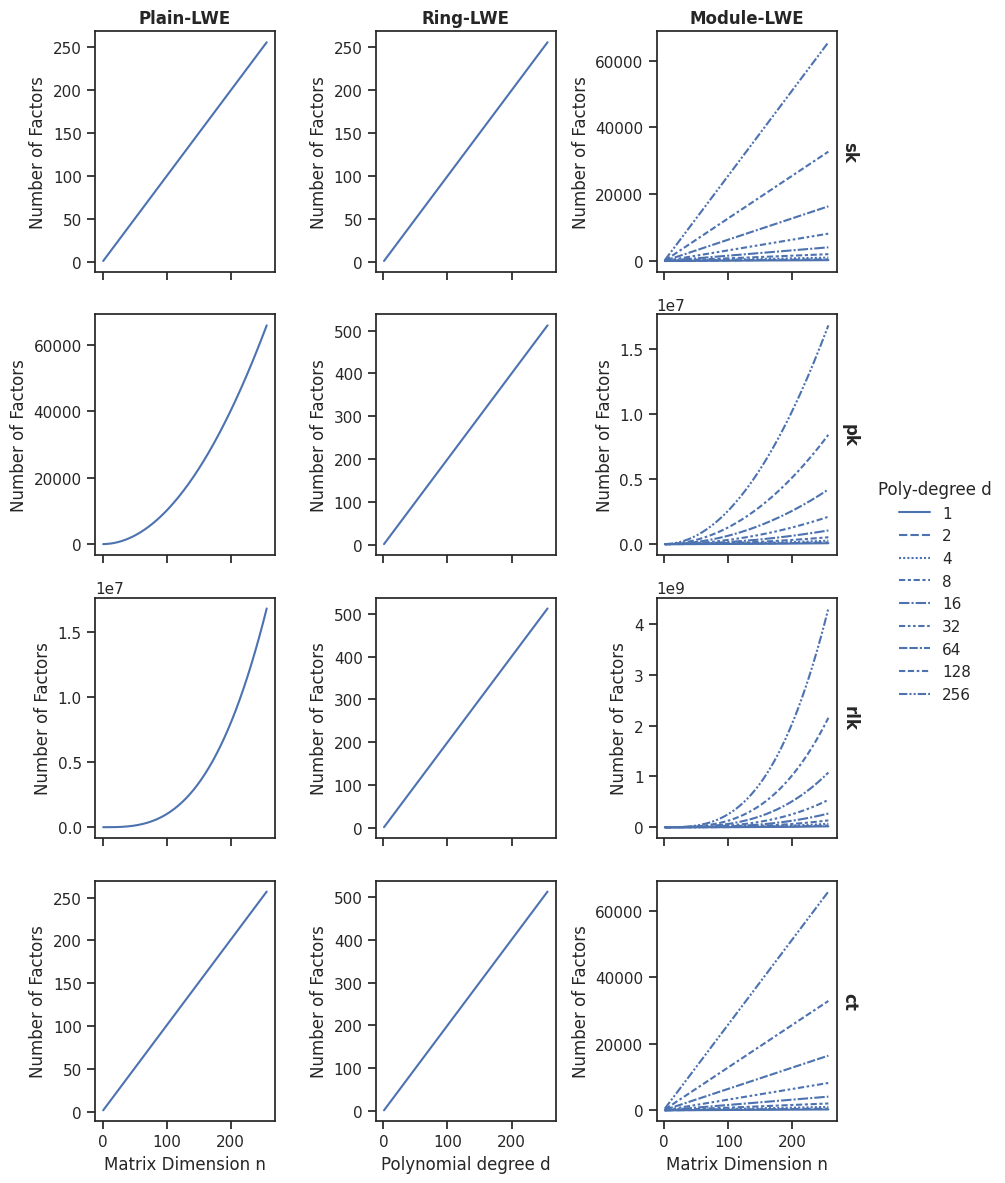
\includegraphics[scale=0.52]{images/OutputFactors.png}
  \caption[Output Variable Factors by Scheme]{The graph illustrates the growth in the number of factors (y-axis) against the dimensions (x-axis). Each of the three columns of plots represents a distinct scheme, as indicated at the top of the figure. The rows represent the output variables, which are indicated on the right-hand side of the right plot. In Plain-LWE and M-LWE, the x-axis is represented by the variable $n$. In contrast, R-LWE employs the variable $d$. In the case of M-LWE, the diverse line types serve to differentiate between distinct values of $d$.}
  \label{fig:OutputFactors}
\end{figure}

The growth rates observed for the secret key $sk$ are linear with regard to the variables $n$ and $d$ for Plain-LWE and R-LWE, respectively. M-LWE exhibits a linear relationship with either $n$ or $d$. When both variables grow simultaneously, the growth rate becomes quadratic. As a consequence, the growth rate for the number of factors in this case exhibits a significantly higher rate of increase than that observed for the other two schemes.

The linear growth rate observed for R-LWE remains for both the private key $pk$ and the relinearization key $rlk$, but with an steeper incline. In contrast, the growth rates for the other two schemes exhibit a significant increase, particularly with regard to the matrix dimension $n$. For Plain-LWE the growth rate of the private key $pk$ is quadratic, while for the relinearization key $rlk$, it is even cubic. When increasing the polynomial degree $d$ simultaneously, the growth rate for M-LWE becomes cubic or quartic, respectively. It is also noteworthy that the $rlk$ does not employ the conventional modulus $q$, as all the other parameters do, but rather the larger modulus $q\cdot p$. As both moduli are represented in the computer as binary numbers, the maximum space they require can be expressed as $2^{q_b}\cdot 2^{p_b} = 2^{q_b+p_b}$. Therefore, rather than requiring $q_b$ bits, it is necessary to use $q_b+p_b$ bits to represent each factor for the $rlk$. This contributes to the unfavorable growth rates observed in Plain-LWE and M-LWE, as more and significantly larger numbers are needed.

The ciphertext $ct$ exhibits a similar growth pattern to that of the secret key $sk$. For Plain-LWE and M-LWE, the growth behavior is nearly identical, with the sole distinction being that, rather than $n$, $n+1$ is utilized. This is negatable when $n$ is increasing. As $n=1$ for R-LWE, the increment of $1$ results in a doubling of the requisite number of parameters, thereby causing the incline to be of the double-value, yet the growth rate remains linear.

One important note that need to be done, is the difference between word-wise and bit-wise FHE schemes \cite{WordBitWiseFhe}. The difference is, that bit-wise FHE operates at the single bit level and word-wise FHE operates on the whole word (eg, 64 bit). This means that each polynomial can be seen as a word and operations can be done all at once and the polynomial dimension $d$ defines the word size. For a bit wise scheme, the logic needs to be done bit wise, which means that a lot more operations need to be done, which makes bit-wise slower. In this thesis, BFV was chosen as backbone for the created M-LWE HE scheme, which is a word-wise scheme, but by choosing $d=1$ it is essentially turned into a bit-wise scheme. In practical terms, this implies that R-LWE and M-LWE are capable of encrypting an entire word at once, for example, 32- or 64-bit numbers. In contrast, Plain-LWE requires that each bit be encrypted individually. This necessitates the decomposition of words into their constituent bits, followed by their encryption and the construction of operations based on these single-bit ciphertexts. This approach not only demands greater computational resources but also requires more memory. Further advantages and disadvantages are detailed in reference, \cite{WordBitWiseFhe}. 

In general, R-LWE requires the fewest number of factors and the smallest amount of physical space to store its output variables. In comparison, Plain and especially M-LWE require a greater number of factors and a greater amount of physical space. Furthermore, the growth rate for R-LWE is significantly lower than that of Plain and M-LWE. In defense of M-LWE, it should be noted that in practice the matrix dimension $n$ is quite small. In the CRYSTALS-Kyber scheme \cite{CyrstalsKyber}, the values are set between 2, which corresponds to low security, and 4, which corresponds to high security. This can be achieved because the security of the system is not solely dependent on the matrix, but also on the polynomials. In contrast to Plain-LWE, significantly larger values of $n$ are required for security. In the Frodo encryption scheme \cite{frodo}, which utilize Plain-LWE, values between $352$ for low security and $864$ for high security and a value of $n=752$ is recommended. This results in the number of factors exceeding $400$ million just for the $rlk$.

A comparison of the physical space required for the various encryption schemes, with variables based on the regular/recommended security level of published encryption schemes that employ the underlying method, can be found in Table \ref{table:OutputVariableInKB}. It is important to note that the results should be interpreted with caution and that direct comparisons between the numbers are not possible. However, the data provides a general indication of the differences between the schemes. Notably, the variables for Plain-LWE are considerably larger than those for the other two, requiring more than$3$ gigabytes, solely for the RLK. Even tho the ciphertext $ct$ is the smallest for Plain-LWE, this amount of disk space is necessary for each bit, whereas R-LWE and M-LWE can store $512$ or $256$ bits, respectively, with a slightly larger $ct$. With the exception of the ciphertext, R-LWE has the smallest overall size for every variable. However, as it can store twice the information of M-LWE and, as previously mentioned, $512$ times more than Plain-LWE, it requires the smallest amount per bit stored.

\begin{table}[h]
  \centering
  \caption[Theoretical LWE HE output variable sizes]{Theoretical LWE Output Variable size in Kilobyte (KB), based on variables for the regular/recommended security level of published encryption schemes. The modulus $p=q^3; p_b=q_b*3$ as used in \cite{bfv}}
  \begin{tabular}{|l|c||c|c|c|c||c|c|c|c|}
    \toprule
              & Source                      & $n$   & $d$   & $q$      & $q_b$ & $sk$    & $pk$      & $rlk$    & $ct$    \\
    \midrule
    Plain-LWE & \cite{frodo}                & $752$ &       & $32767$  & $15$  & $1.41$  & $1061.73$ & $3193684$ & $1.41$ \\
    R-LWE     & \cite{PracticalKeyExchange} &       & $512$ & $25601$ & $15$  & $0.96$  & $1.92$    & $7.68$   & $1.92$  \\
    M-LWE     & \cite{CyrstalsKyber}        & $3$   & $256$ & $7681$   & $13$  & $1.25$ & $4.992$   & $59.904$ & $1.66$ \\
    \bottomrule
  \end{tabular}
  \label{table:OutputVariableInKB}
\end{table}

In conclusion, the comparison based on the size of the output values indicates that R-LWE has the slowest growth of physical space needed based on its dimension variables. Although M-LWE has the fastest growth rate, as it is based on multiple dimension variables, this makes it far more secure than Plain-LWE. Consequently, the dimensions can be smaller in general to achieve a similar level of security, which results in a smaller physical size of its output variables. In terms of storage requirements for the output variables, Plain-LWE is by far the most demanding, with M-LWE requiring more physical space than R-LWE. However, the difference in these requirements is not as significant as that observed in the comparison with Plain-LWE.

\section{Time cost comparison}

The objective of this section is to perform a comparative analysis of the runtime performance of the algorithms with respect to a selected set of input parameters. To minimize the impact of noise, multiple iterations of each algorithm were executed with the specified inputs, and the median time value in seconds was calculated. In total, there are four parameters that can be manipulated: the dimensions $n$ and $d$, as well as the modulus values $q$ and $p$. To simplify the analysis of multiple variables and enhance the visualization of the differences, two performance tests were conducted. One test was conducted with varying dimension variables $n$ and $d$, while the modulus values $q$ and $p$ were constant. The second test was performed with the variables $n$ and $d$ fixed while the modulus values $q$ and $p$ were allowed to vary. This should provide a more straightforward means of illustrating the impact of these variables on the performance of the algorithms. The algorithms that are evaluated are the \textit{KeyGen} (Algorithm \ref{alg:HomomorphKeyGen}), the \textit{Encryption} (Algorithm \ref{alg: SampleLweEncryption}), the \textit{Decryption} (Algorithm \ref{alg: SampleLweDecryption}), the \textit{Addition} (Algorithm \ref{alg:MlweAddition}) and the \textit{Multiplication} (Algorithm \ref{alg:moduleMultiplication}).

The initial comparison is that of processing time, based on the two size dimensions, namely, $n$ and $d$. The results of the comparative analysis of the algorithms' performance are presented in Figure \ref{fig:nd-performance}. 

\begin{figure}[ht!]
  \centering
  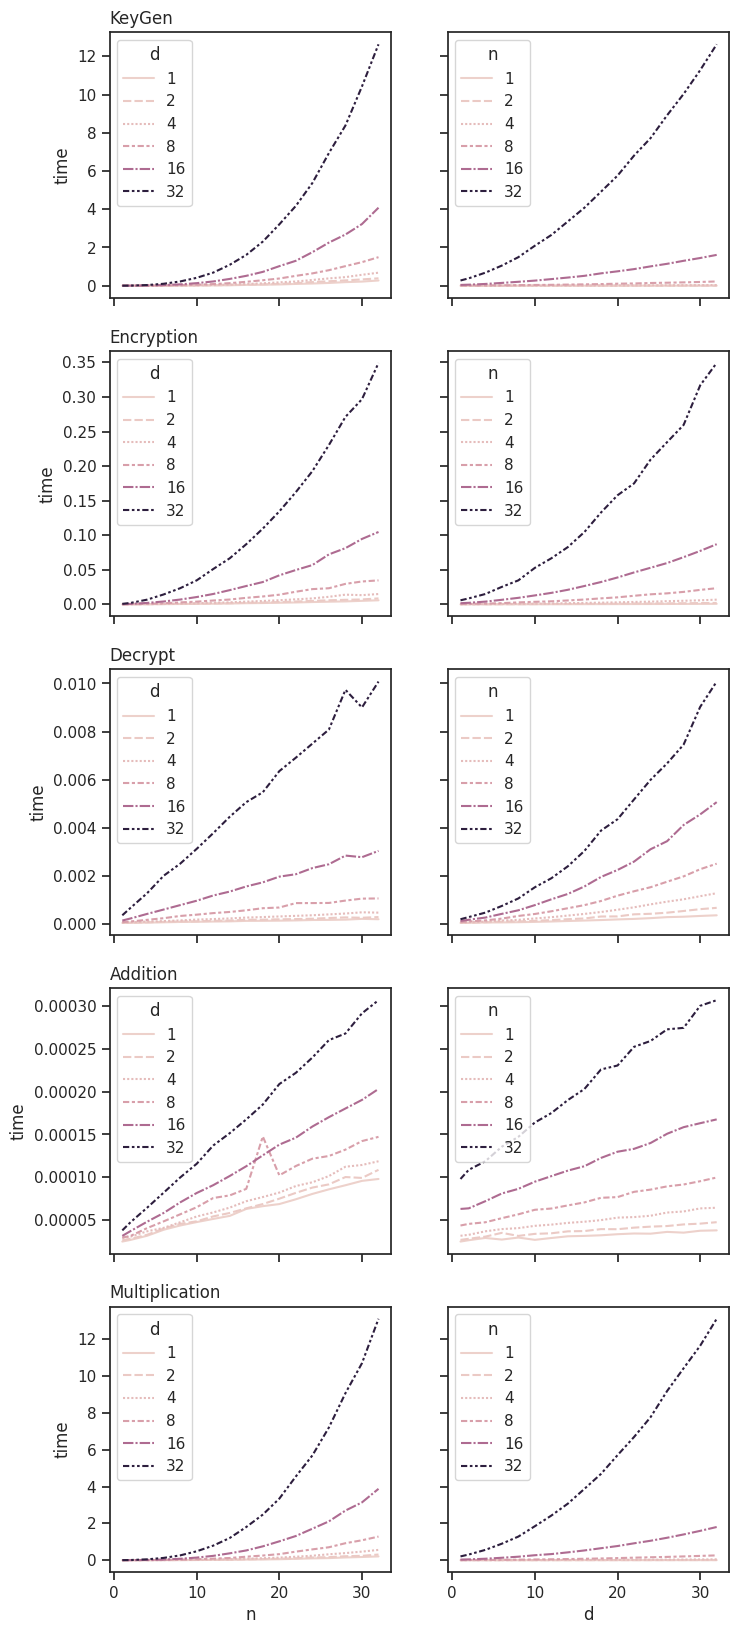
\includegraphics[scale=0.5]{images/nd-performance.png}
  \caption[Performance of the HE algorithms by $n$ and $d$]{Performance of the main algorithms in regard to dimensions $n$ and $d$ and the time in seconds. Each row is a different function, as stated always above the left plot. The left column plots the time against $n$ for some $d$ values. The right column plots the time against $d$ for some $n$ values.}
  \label{fig:nd-performance}
\end{figure}

In the figure, Plain-LWE is illustrated in the left column, in the line representing $d=1$, and R-LWE is shown in the right column with $n=1$. All other lines represent distinct versions of M-LWE. It can be observed that the \textit{KeyGen} and \textit{Multiplication} algorithms are the most time-consuming. Regardless of whether $n$ or $d$ is increased, these algorithms exhibit an exponential growth in time cost. However, the rate of increase for $d$ is relatively modest, in contrast to the significant rise observed in the case of $n$. This exponential growth can be attributed to the fact that, in order to perform matrix multiplication, the number of scalar multiplications increases quadratically. One potential solution to this issue is the use of dedicated matrix multiplication hardware, which performs the entire operation in a single step, or the incorporation of other optimized libraries. In order to work with numbers greater than 64 bits, it was not feasible to utilize the aforementioned libraries in the implemented system. Consequently, arbitrary-size integers in pure Python were employed, which yielded the observed outcomes. This provides an explanation as to why the increase of $n$ results in exponential Growth, but also demonstrates that this phenomenon occurs at a slower rate when $d$ is increased. The rationale behind this approach is that, in order to perform polynomial multiplication, the methodology outlined in Section \ref{sec:PolyMulMath} was employed, which translates polynomial multiplication into matrix-vector multiplication. As the value of $d$ increases, the dimensions of the matrix also increase, resulting in a quadratic growth in the number of multiplications required, following the same pattern previously described. The combination of these two facts also explains why the growth for $n$ is more pronounced. In addition to the increase in the number of polynomial multiplications due to the larger dimensions, each new polynomial multiplication also exhibits a quadratic runtime.
As the number of matrix multiplications increases, the algorithms become less efficient, exhibiting a decline in speed. This phenomenon is most evident in the \textit{KeyGen} and \textit{Multiplication}, where a single matrix multiplication is required for each $rlk$, which increases linearly with $n$. Consequently, these algorithms are quite slow. The \textit{Encryption} algorithm requires only a single matrix-vector and one vector-vector multiplication, resulting in a quadratic growth rate. This makes it significantly faster than the previously mentioned algorithms. In contrast, \textit{Addition} does not require any multiplication, making it the fastest algorithm by far. As only vectors need to be added, the time growth is also linear, as the number of additions scales linearly with the size of the vectors. With the \textit{Decryption}, there is a very interesting pattern. While the runtime scales linearly with the increase of $n$, it has a quadratic growth with the increase of $d$. This is due to the quadratic scaling of the matrix required for the polynomial multiplication, as previously explained.

In consideration of the overall performance, the impact of input parameters can result in a significant decline in performance, potentially by a factor of multiple and even orders of magnitude. Therefore, the input dimensions exert a considerable influence on the performance.

\begin{figure}[ht!]
  \centering
  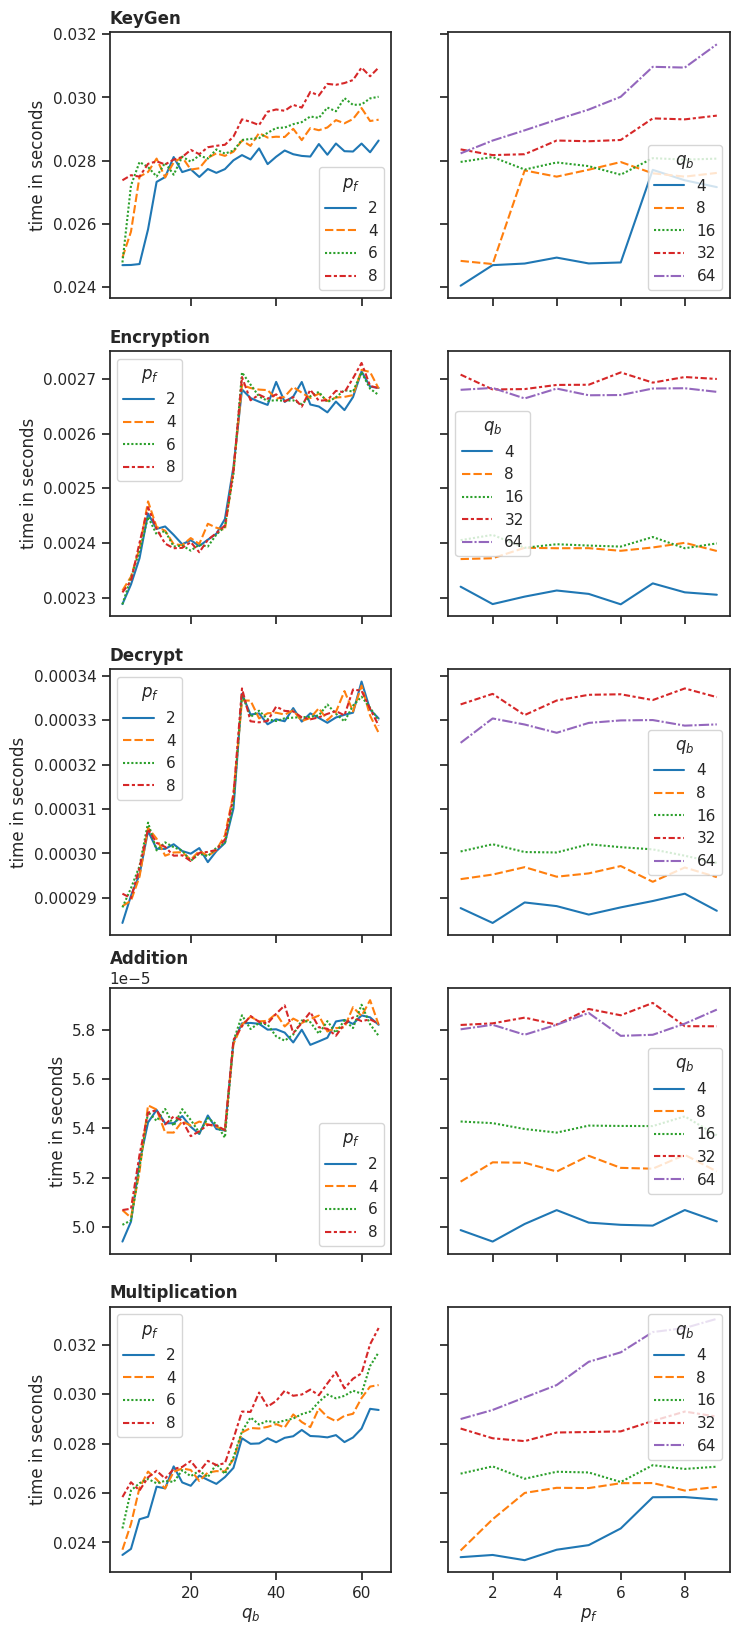
\includegraphics[scale=0.48]{images/qp-performance.png}
  \caption[Performance of the HE algorithms by $q$ and $p$]{Performance of the main algorithms in regard to modulus with $q$ and the modulus factor $p$, which represents $q*p$ bit in regards to the time in seconds. Each row is a different function, as stated always above the left plot. The left column plots the time against $q$ for some $p$ values. The right column plots the time against $p$ for some $q$ values.}
  \label{fig:qp-performance}
\end{figure}

The second cost comparison is based on the development of the modulus $q$ and $p$, as illustrated in Figure \ref{fig:qp-performance}. 
The quantity represented by the variable $q$ in the graph is the number of bits for the modulus $q_{mod} = 2^q$, while the quantity represented by the variable $p$ is the factor by which the $q$ bits are multiplied to retrieve the modulus $p_{mod} = 2^{q*p}$. The rationale for this is that the value of $p$ should be a multiple of several orders of magnitude greater than that of $q$, as outlined in the BFV paper \cite{bfv}. To more clearly illustrate the outcomes, the factors are presented instead of the actual modulus values. Consequently, the x-axis employs a logarithmic scale rather than a linear one.

When looking at all graphs, there are two Groups, KeyGen and Multiplication, which have a linear increase in time consumption and the others, which seem to have steps and between the steps a constant time consumption, when increasing $q$. The big difference between these two groups is, that the first group needs $p$ for computations, while the others only using $q$.  This is also the reason why for the right graphs for group one there is a linear increase with the increase of $p$ and for group two it stays constant. When looking at group two, on the left side, there can be seen performance jumps around $16$ and $32$ bits. The case could be that python has some internal improvements for $16$ bit and $32$ bit numbers. For the first group, this is not the seen, as they calculate always with numbers greater then $32$ bits, because of the usage of $p$.

Upon examination of the data, it becomes evident that there are two distinct groups of algorithms: KeyGen+Multiplication and Encryption+Decryption+Addition. The former exhibits a linear increase in time consumption, while the latter displays a pattern of steps and a constant time consumption between steps, as $q$ increases. The primary distinction between these two groups is that the former requires the use of $p$ for computations, whereas the latter employs solely $q$.  This is also the reason why, for the right graphs associated with group one, there is a linear increase with the increase of $p$, whereas for group two, this value remains constant. Group two, on the left side, exhibits performance jumps around $16$ and $32$ bits. It is plausible that Python has internal improvements for $16$ and $32$ bit numbers. However, this is not observed in the first group, as they calculate with numbers greater than $32$ bits due to the usage of $p$.

In general, it can be observed that the variables $q$ and $p$ exert a relatively minor influence on performance, particularly in comparison to the dimension variables. As evidenced by the data, even a significant discrepancy in $q$ and $p$ only results in a $40\%$ increase in the time required for multiplication. However, when considering the range of $p$ values, from $4*10=40$ bits to $80*10=800$ bits, the observed increase is a factor of $20$.


\begin{table}[h]
  \centering
  \caption{M-LWE and R-LWE Performance in seconds, based on variables for the regular/recommended security level of published encryption schemes}
  \begin{tabular}{|l|c||c|c|c|c|c|}
    \toprule
          & Source                      & Addition & Decrypt  & Encryption & KeyGen   & Multiplication \\
    \midrule
    R-LWE & \cite{PracticalKeyExchange} & 0.000163 & 0.061521 & 0.125041   & 0.182526 & 0.473052       \\
    M-LWE & \cite{CyrstalsKyber}        & 0.000176 & 0.041224 & 0.174293   & 0.696122 & 1.039662       \\
    \bottomrule
  \end{tabular}
  \label{table:performanceComparison}
\end{table}

To provide some real-world examples, the same parameters as in the previous section (see Table \ref{table:OutputVariableInKB}) were used to calculate the performance in seconds, which can be seen in Table \ref{table:performanceComparison}. The Plain-LWE version was excluded from the comparison due to the discrepancy between the required memory and the available memory, which prevented its execution. Even if the limitation could be overcome, the runtime would be significantly slower than that observed for the other two versions. A comparison of the two remaining cases reveals that they both operate within the same order of magnitude. With the exception of the decryption algorithm, the R-LWE algorithms are consistently faster than their M-LWE counterparts. This discrepancy in decryption time may be attributed to the fact that R-LWE has twice the polynomial degree $d$, compared to M-LWE. But this also means, that R-LWE works with the double word size at the same time, which allows for bigger numbers to be operated on. Additionally, it is not unexpected that the M-LWE version is slower than R-LWE, as the higher matrix dimension, $n$, necessitates more calculations.

As previously demonstrated, the majority of algorithms exhibit a quadratic growth in runtime with respect to the dimension variables, namely $n$ and $d$. This is growth rate is especially problematic for KeyGen, which has the advantage of being executed only once per session, and for multiplication, which is a significant challenge for homomorphic encryption schemes. In order to maintain satisfactory performance, it is advisable to minimise the dimensions, with particular attention paid to the matrix dimension $n$, which exhibits a higher growth rate and therefore a greater influence. In contrast, the influence of the modulus $q$ and $p$ on performance is comparatively minor, particularly in comparison to the dimension variables. Thus, increasing these variables results in a slight decline in performance, but not a drastic one. When examining real-world parameters, it becomes evident that R-LWE remains the most optimal choice, closely followed by its M-LWE counterpart. Plain-LWE exhibits a considerable memory footprint, which would also result in a significant decline in performance, rendering it impractical to run this version at all in practice.

\section{Comparison of the additive and multiplicative depth}

As the number of operations performed in a homomorphic manner increases, the resulting error grows in magnitude. After a certain number of operations, the accumulated error becomes so significant that the decryption process yields incorrect numerical values. The source of the error is the ciphertext itself, which is the foundation of LWE's security. This section will examine the maximum depth and the extent of the error growth for addition and multiplication operations, as well as the impact of dimension variables $n$ and $d$, and modulus variables $q$ and $p$.

The following statistical data were derived from a process whereby an operation was performed repeatedly with a given ciphertext. The initial step involved encrypting a randomly generated message, thereby creating the original ciphertext. In each iteration, a new, randomly generated message was encrypted, resulting in a distinct ciphertext. Subsequently, the newly generated ciphertext was added or multiplied, depending on the specific test, to the original message, thereby updating it. Subsequently, the updated ciphertext was evaluated to ascertain whether the resulting message, obtained through decryption, exhibited the same outcome as if the calculations had been performed in plaintext space. Subsequently, the discrepancy between the present ciphertext and the correct plain text, the error, was recorded for each iteration.
This process is then repeated until either the decrypted message does not match the expected result or until a pre-defined maximum limit is reached, as otherwise the procedure would take an excessive amount of time. For each parameter set, this process was repeated multiple times to reduce noise. The median values for each round were then calculated. The rounds are referred to as depth, which denotes the number of consecutive operations that can be performed.

First, the additive depth and error will be subjected to examination. The graphs illustrating this can be seen in Figure \ref{fig:AddErrorDev}. The addition is dependent on three variables: the two dimensional variables and the modulus, $q$. The modulus $p$ is not a required component of the addition process and therefore does not exert any influence on it. The figure illustrates the evolution of the error with depth for various configurations of the dimensions and for different modulus values. Once more, the value of $q$ represents the exponent, and the utilized modulus is defined as $q_{mod} = 2^q$. The error axis is logarithmic in order to facilitate the visualization of the comparative magnitude of the errors. A logarithmic curve is observed in nearly all of the graphs, indicating that the error grows in a linear fashion with depth. In the event that the value of $q$ is insufficient, the curve will be terminated prematurely, as the resulting error is too high for successful decryption. As the value of $q$ increases, the minimum error decreases, thereby enabling a greater number of operations. However, when $n$ or $d$ are increased, the minimum error rises due to the number of total factors and with that more error in the system. Accordingly, as the dimensions increase, a larger modulus must be selected to facilitate subsequent additions. The linear growth can be attributed to the fact that the errors resulting from the addition are simply added together, as outlined in algorithm \ref{alg:MlweAddition}. Therefore, the resulting error is equal to the sum of the two errors from the ciphertexts. In this experiment, only freshly encrypted data with a minimal error was added to one ciphertext. In practice, however, ciphertexts with larger errors will also be added, as they will have undergone previous operations. When the errors are combined, the growth rate will be faster than that shown in the graph. Nevertheless, the growth rate remains linear and thus manageable and with a sufficiently large modulus, which makes it possible to run more then $200$ additions easily, as can be seen by the error in the graphs. Also the maximum used modulus with $q_mod = 2^{32}$, is not that high and bigger ones could be used without any problem making it possible to run more than $1000$ additions in a row.

\begin{figure}[ht!]
  \centering
  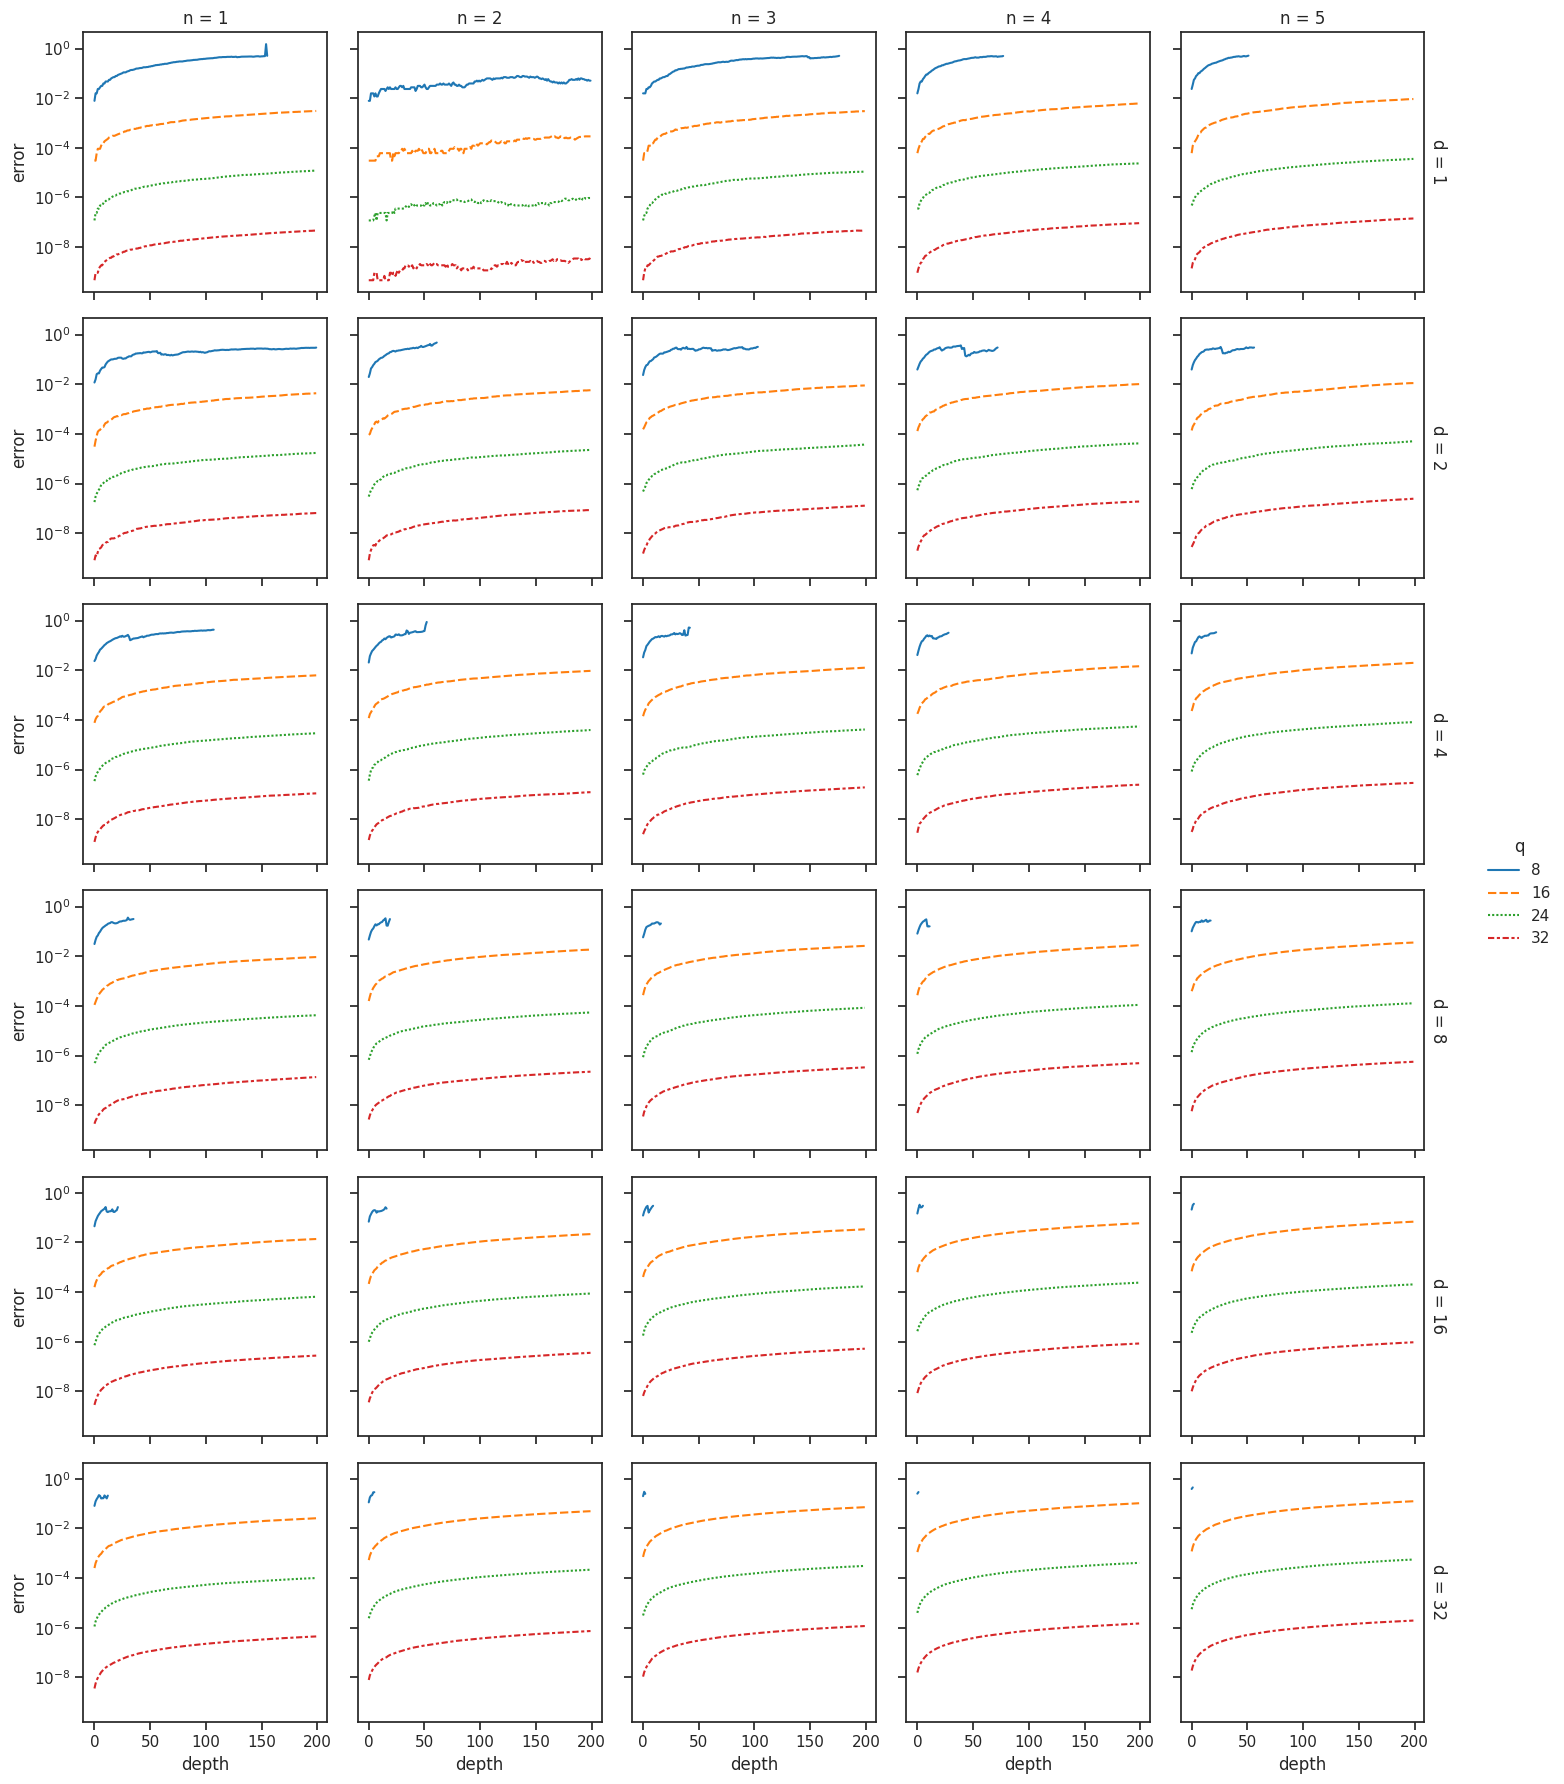
\includegraphics[scale=0.38]{images/AddErrorDevelopment.png}
  \caption[Additive Error Development]{Additive Error Development}
  \label{fig:AddErrorDev}
\end{figure}

A comparison of the various LWE schemes reveals that the difference in computational depth for addition is not significant when evaluated based on depth alone. A comparison of the associated data indicates that the variables $n$ and $d$ exert a comparable influence on the reduction of computation depth. Consequently, an evaluation of the graphs suggests that Plain-LWE and R-LWE exhibit comparable performance for small dimensions. M-LWE, however, which incorporates both $n$ and $d$ into its formulation,results in a lower computational depth for addition.


The next step is to analyse the multiplication process, which is illustrated in Figure \ref{fig:MulErrorDev}. The multiplication function makes use of the modulus $p$ for the modulus switching component. The impact of this variable is illustrated by the colored bands displayed alongside each graph. It displays the minimum to maximum error values for all values of $p$ at that depth. To obtain a comprehensive set of values, multiple runs were conducted with identical dimension variables and modulus, and varying $p$ values between $1$ and $15$. This resulted in the calculation of the modulus $p_{mod}=2^{q*p}$. The primary line represents the median values for a given depth across all $p$ values.

\begin{figure}[ht!]
  \centering
  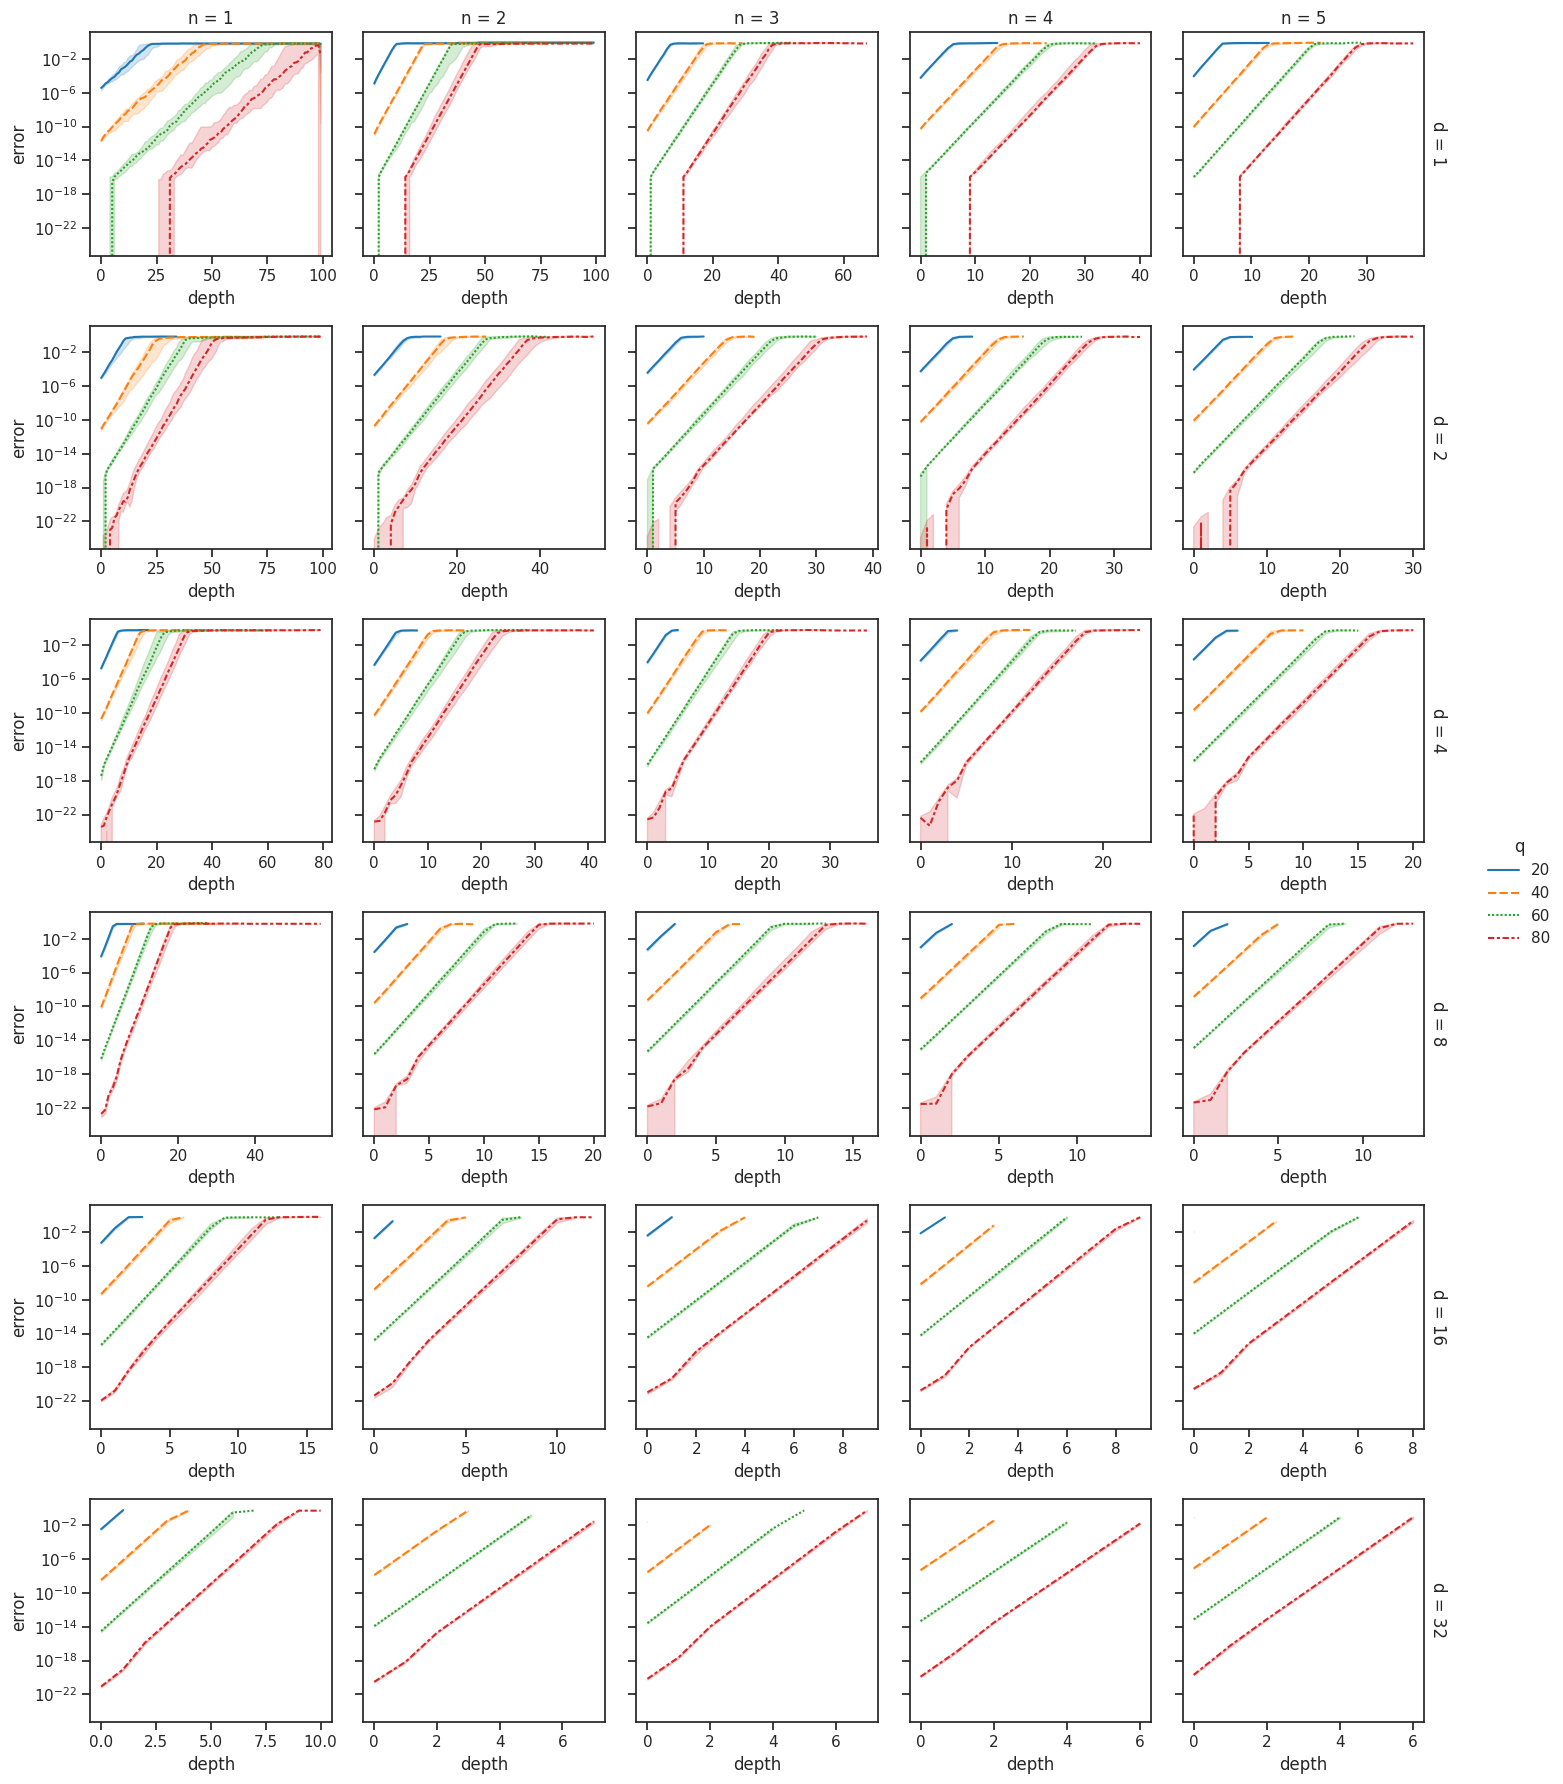
\includegraphics[scale=0.38]{images/MulErrorDevelopment.png}
  \caption[Multiplicative Error Development]{Multiplicative Error Development}
  \label{fig:MulErrorDev}
\end{figure}

In contrast to the behavior observed in the addition function, the error line in these graphs is, in general, more linear. As the error axis employs a logarithmic scale, the error grows exponentially with each multiplication. This results in a relatively shallow depth, particularly when the dimensions are increasing. To illustrate, the maximum depth attained in the bottom rightmost graph is $6$, with an modulus of $q_{mod} = 2^{80}$. The aforementioned error growth is also elucidated in other studies regarding LWE-based FHE schemes. For instance, in reference \cite{FHEwoBottstrapping}, it is detailed that the error for addition increases by a maximum of two, while for multiplication, the error is quadratic in the worst case. These analogous growth rates are observable in the graphs for addition and multiplication.

The value of $p$ is utilized for the modulus switching process, with the objective of enabling multiplication and concurrently reducing the error, as detailed in reference \cite{bfv}. As evidenced by the graphs, this objective was not achieved for any value of $p$. Furthermore, an additional trial was conducted, wherein the value of $p$ was increased to a considerably higher amount, specifically $1000$. This resulted in the generation of a modulus with a size of $2^{q*1000}$. However, this approach did not yield any apparent improvement in the outcomes observed for the higher-dimensional m-lwe schemes, such as the one depicted in the bottom right region of the graph. The precise reason why $p$ has no tangible impact is yet to be determined. One potential explanation for this discrepancy is the presence of numerical issues and minor rounding errors associated with the manipulation of these large numbers in the Python. In particular, the process of dividing by $p$, as illustrated in steps $4$ and $5$ of algorithm \ref{alg:moduleMultiplication}, may introduce minor rounding errors due to the conversion from an arbitrary-size integer to a $64$-bit float. This could potentially contribute to the observed issue.

When comparing the influence of the variables $n$ and $d$ and, consequently, the various schemes, on the multiplication error and depth, it becomes evident that, as was the case with addition, both variables exert a roughly equivalent influence. Therefore, irrespective of the variable that is increased, the computational depth rate will decline to a similar extent. As observed in the case of multiplication and addition, by enhancing the modulus $q$, the minimum error can be lowered, consequently leading to an increase in the computational depth. This phenomenon occurs for all operations due to the intrinsic nature of the scheme itself, rather than the specific operation, and thus was to be expected.

\begin{table}[h]
  \centering
  \caption[M-LWE and R-LWE computation depth comparison]{A comparison of the computation depth of M-LWE and R-LWE for variable modules, with $q_{mod} = 2^q$ and $p_{mod}=2^{q*3}$. The remaining parameters are based on variables corresponding to the regular or recommended security level of published encryption schemes. The resulting numbers are the median values when an error occurred and thus it no further calculations were possible.}
  
  \begin{tabular}{|cc|rrrrrr|rrrrrr|}
    \toprule
                                       &   & \multicolumn{6}{|c|}{Addition} & \multicolumn{6}{|c|}{Multiplication}                                                        \\
                                       & q & 13                             & 15                                   & 20  & 32  & 64  & 128 & 13 & 15 & 20 & 32 & 64 & 128 \\
    \midrule
    R-LWE  \cite{CyrstalsKyber}        &   & -                              & 56                                   & 200 & 200 & 200 & 200 & -  & 0  & 0  & 1  & 3  & 7   \\
    M-LWE  \cite{PracticalKeyExchange} &   & 7                              & -                                    & 200 & 200 & 200 & 200 & 0  & -  & 0  & 1  & 3  & 7   \\
    \bottomrule
  \end{tabular}
  \label{table:depthComparison}
\end{table}

As a final comparative analysis, the R-LWE and M-LWE algorithms were once again evaluated with the aid of a number of recommended parameters. The outcome of this comparison is presented in Table \ref{table:depthComparison}. In order to evaluate the computational feasibility of the proposed approach, the experiment was conducted with increased modulus values. Both the M-LWE and R-LWE versions are capable of performing addition in their base configurations, however, the depth for the R-LWE is considerably higher than that for the M-LWE. However, it was not possible to perform multiplication for any scheme with the original modulus values. As the value of $q$ increased, the depth for addition could be easily raised to the maximum depth for this comparison ($200$) for both schemes in an equal manner. Achieving the desired increase in depth for multiplication proved more challenging. With a modulus of $128$-bits, only an average of seven computations in a row were feasible. However, the values observed between the models are identical, indicating that the error increase is approximately equivalent across both R-LWE and M-LWE. In general it can be seen, that the R-LWE and M-LWE schemes are quite similar in additive and multiplicative depth for the same modulus $q$.

As discussed before, with a polynomial dimension $d$ for R-LWE that is twice that of M-LWE, R-LWE is capable of processing significantly larger numbers.

\info[inline]{Evtl nochmal ein paar werte aus den Graphen raussuchen und genauer gegenüber stellen. Z.b wie verändert sich der Fehler nach 3 multiplikationen für verschiedene q werte.}